\documentclass[aspectratio=169]{beamer}
%package
\usepackage[utf8]{inputenc}
\usepackage[T1]{fontenc}
\usepackage{tikz}
\usepackage{appendixnumberbeamer}

\usetheme[showmaxslides,darkmode]{pureminimalistic}

\renewcommand{\appendixname}{\texorpdfstring{\translate{appendix}}{appendix}}
% no logos
\renewcommand{\logofooter}{}
\renewcommand{\logotitle}{}
\renewcommand{\logoheader}{}

\title[Portfolio] {Portfolio}
\author{Emmanuel Vera}
\institute{Senior Electronics Engineer}
\date{\today}


\begin{document}

\maketitle

\begin{frame}[plain, noframenumbering]{Outline}
  \tableofcontents
\end{frame}

\section{Mastrack}
\begin{frame}{Mastrack}
  OBD interface car sensor board that records and transmit data. It uses a 
  STM32 microcontroller and a BG95 quectel module.
  \begin{figure}[H]
    \centering
    \begin{columns}[T]
      \begin{column}{.3\linewidth}
        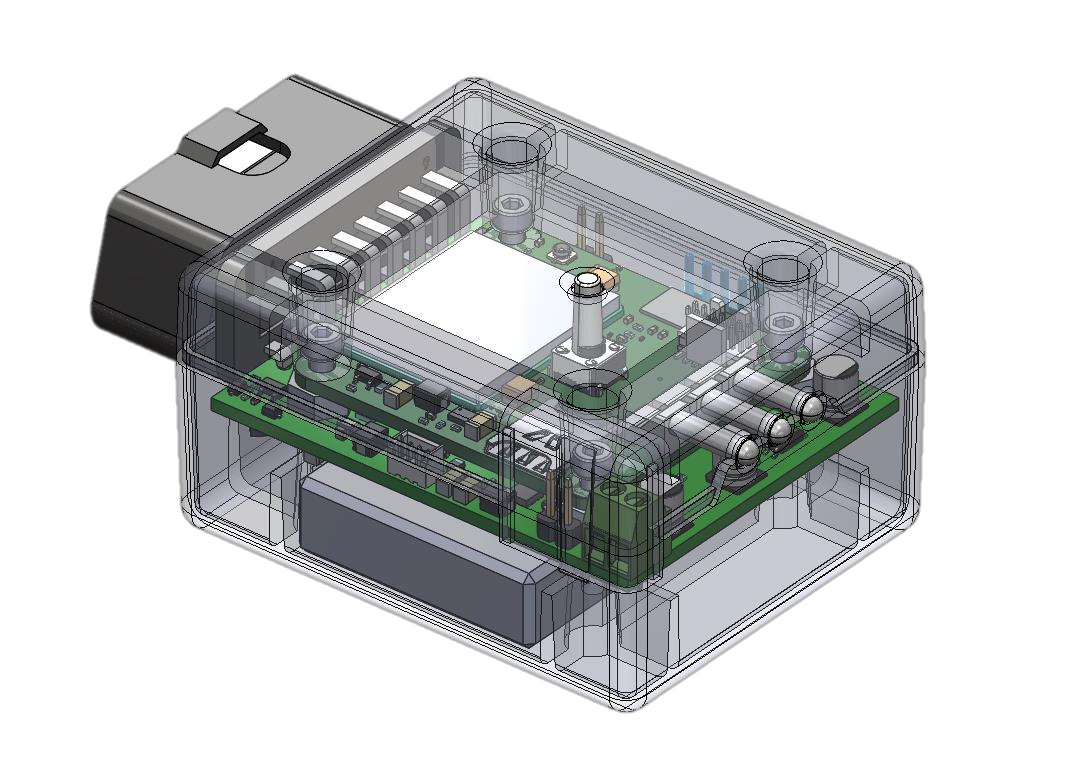
\includegraphics[width=\linewidth]{images/Mastrack1}
      \end{column}
      \begin{column}{.3\linewidth}
        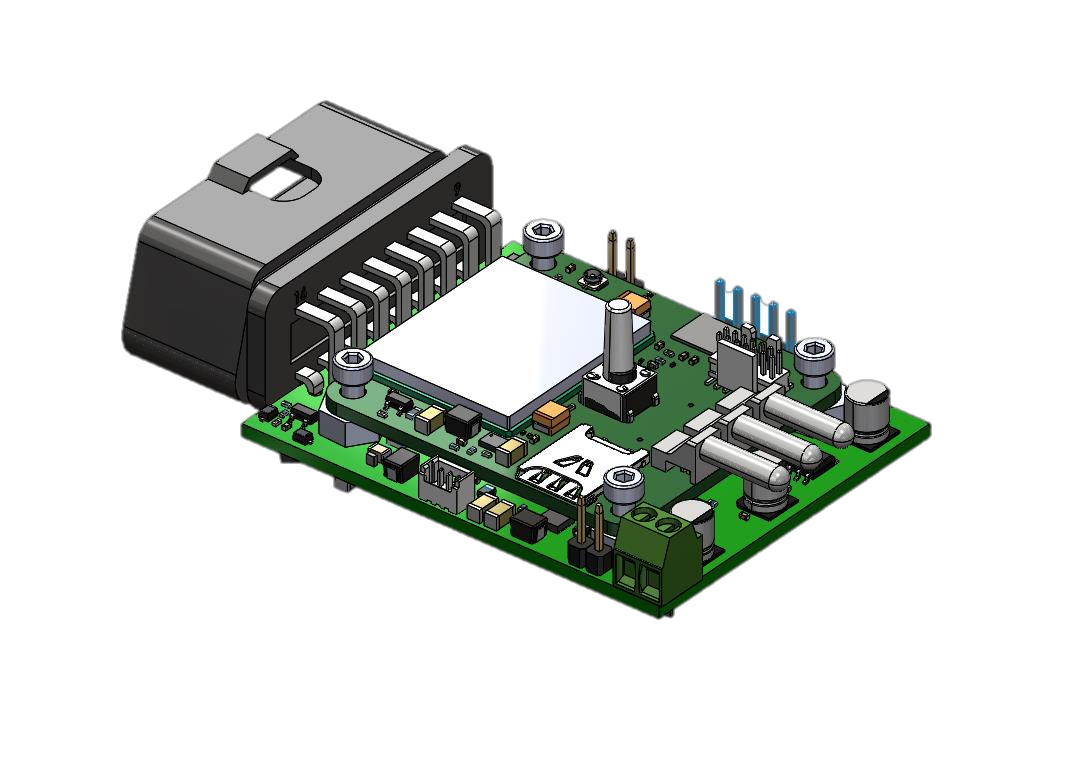
\includegraphics[width=\linewidth]{images/Mastrack2}
      \end{column}
    \end{columns}
  \end{figure}
\end{frame}

\end{document}
